\RequirePackage{fix-cm}
\makeatletter
\def\@journalname{Journal of Real-Time Image Processing}
\makeatother
\documentclass[twocolumn]{svjour3}
\smartqed
\usepackage{graphicx}
\usepackage{amsmath,amssymb,amsfonts}
\usepackage{textcomp}
\usepackage{booktabs}
\usepackage{array}
\usepackage{url}
\graphicspath{{figures/}}

\journalname{Journal of Real-Time Image Processing}

\begin{document}

\title{Real-Time Stage-Level Evaluation of SIMD-Native Chaos-Based Image Encryption Pipelines}
\titlerunning{Real-Time Evaluation of Chaos-Based Image Encryption}

\author{Ravikanth Reddy Gudipati}
\authorrunning{R. R. Gudipati}

\institute{Ravikanth Reddy Gudipati \at
University at Buffalo, Buffalo, NY, USA \\
\email{ravikanthreddy@ieee.org}}

\date{}

\maketitle

\begin{abstract}
Chaos-based image-encryption studies commonly report aggregate running time
and image-domain statistics, but often do not show whether the proposed
pipeline can satisfy real-time image-processing budgets or which stage prevents
it from doing so. This work presents a reproducible C++17 benchmark that
decomposes representative chaotic image-encryption methods into keystream
generation, pixel permutation, and diffusion, then evaluates end-to-end
latency, throughput, and stage share against frame-rate constraints.
Traditional components are compared with SIMD-oriented replacements on
synthetic images, Kodak PhotoCD images, and a public 720p/1080p video-frame
workload. The real-time extension adds matched x86-64 and ARM64 video-frame
measurements with mean latency, p95 latency, FPS-equivalent throughput, and
30/60 FPS feasibility labels. Replacing chaotic sort permutation with a linear
block permutation improves mean permutation throughput by 100.6--131.9 times.
Replacing a global feedback chain with AVX2 multi-lane or tree diffusion
improves mean diffusion throughput by approximately 1.8--2.1 times. The
fastest benchmark-informed candidate, Checkerboard-CA-ARX, sustains 259.1
MiB/s on Kodak images and 200.0 MiB/s at 4096$\times$4096, while ChaCha20
remains substantially faster. Security experiments show that favorable
entropy, histogram, correlation, and key-sensitivity values do not imply
resistance to differential or known-plaintext attacks.
\keywords{chaotic image encryption \and real-time image processing \and SIMD
\and stage-level benchmarking \and permutation-diffusion \and latency}
\end{abstract}

\section{Introduction}
\label{sec:introduction}
Real-time image-processing systems need predictable latency, not
only visually plausible ciphertexts or high aggregate throughput. A
30-frame/s pipeline has about 33.3 ms to process each frame, while a
60-frame/s pipeline has about 16.7 ms before accounting for capture,
transport, display, storage, or downstream analytics. Chaos-based
image-encryption papers often report image-domain statistics and a single
running time, but that evidence rarely shows whether a design can satisfy
these frame budgets on commodity CPU architectures.

The permutation-diffusion architecture is a recurring structure in
chaos-based image encryption. A permutation stage rearranges pixel positions,
and a diffusion stage modifies pixel values using a key-dependent sequence.
The architecture maps naturally to common image statistics: permutation
reduces adjacent-pixel correlation, while diffusion can flatten histograms and
increase sensitivity to key changes.

However, three problems complicate real-time and security claims in this
literature. First, complete-scheme timing hides the contribution of individual
stages. A proposed SIMD diffusion kernel may be fast while an
$O(N\log N)$ chaotic sort still dominates total execution time. Conversely, a
sequential chaotic generator may prevent a pipeline from benefiting from an
otherwise parallel permutation. Second, throughput alone can mask missed
frame deadlines: a high mean MiB/s value is less useful without per-frame
latency, p95 latency on frame sequences, and pass/fail status against 30/60
FPS budgets. Third, image-domain metrics such as entropy, correlation, NPCR,
and UACI are diagnostic measurements rather than proofs of cryptographic
security. A deterministic stream-XOR construction can produce a uniform-looking
ciphertext while remaining vulnerable when a key/nonce pair is reused.

This study investigates how implementation-friendly stages affect the
performance of chaotic image-encryption methods without conflating that
engineering result with cryptographic security. Traditional chaotic
components, SIMD-oriented alternatives, and standard cryptographic baselines
are implemented within one benchmark suite. The experiments isolate keystream,
permutation, and diffusion execution time before composing selected components
into benchmark-informed candidate pipelines.

The study answers five research questions:
\begin{itemize}
\item \textbf{RQ1:} Which stages dominate representative chaotic
image-encryption pipelines?
\item \textbf{RQ2:} Which replaceable stage designs benefit most from
linear-time and SIMD-oriented restructuring?
\item \textbf{RQ3:} Do stage-level improvements remain visible in composed
candidate pipelines and at larger image sizes?
\item \textbf{RQ4:} Which candidates meet 30-frame/s and 60-frame/s latency
budgets at common image and video-frame resolutions on measured CPU
architectures?
\item \textbf{RQ5:} Which security conclusions are, and are not, supported by
common image-domain metrics?
\end{itemize}

The contributions are:
\begin{enumerate}
\item A reproducible C++17/OpenCV/OpenSSL benchmark with a common cipher
interface and separate keystream, permutation, diffusion, and total timing.
\item A real-time evaluation protocol that reports milliseconds per frame,
FPS-equivalent throughput, stage shares, and pass/fail status against 30/60
FPS budgets.
\item A controlled comparison of traditional components and SIMD-oriented
replacements across synthetic images, real natural images, video frames, and
resolutions up to 4096$\times$4096.
\item Evidence that linear block permutation and lane/tree diffusion remove
major implementation bottlenecks, while scalar floating-point maps and
sort-based permutation remain expensive.
\item A negative security result demonstrating that strong image statistics
can coexist with differential and reused-nonce known-plaintext weaknesses.
\item An explicit boundary between fast image-domain transformation prototypes
and cryptographically deployable encryption.
\end{enumerate}

\section{Background and Related Work}
\label{sec:background}

\subsection{Permutation-Diffusion Image Encryption}
Shannon identified confusion and diffusion as fundamental properties of
secret-key systems \cite{shannon1949}. Fridrich adapted related ideas to image
encryption using two-dimensional chaotic maps and a permutation-diffusion
architecture \cite{fridrich1998}. Many later schemes use pixel-, bit-, or
block-level permutation followed by one or more diffusion rounds
\cite{fu2014,huang2018}.

Traditional chaotic permutation often generates one chaotic score per pixel
and sorts pixel indices by those scores. The method is simple to describe but
requires $O(N\log N)$ comparisons and irregular memory access. Diffusion is
frequently implemented as the global recurrence
\begin{equation}
C[i] = P[i] \oplus K[i] \oplus C[i-1],
\label{eq:global-chain}
\end{equation}
where $P$, $K$, and $C$ denote permuted plaintext, keystream, and ciphertext.
This construction creates an apparent avalanche path but also introduces a
loop-carried dependency that restricts vectorization.

\subsection{Chaotic and Spatial Keystream Generators}
Scalar logistic, tent, and sine maps are common keystream sources. Their
iterative dependency and floating-point operations can limit throughput.
Spatial systems such as coupled-map lattices and cellular automata expose
multiple local states and are therefore more compatible with lane-level or
data-parallel execution \cite{chai2015}. This work evaluates both categories,
as well as Hamiltonian-inspired and reaction-diffusion generators.

\subsection{SIMD-Oriented Restructuring}
Single Instruction, Multiple Data (SIMD) instructions operate on multiple
values per instruction. On the evaluated x86-64 host, AVX2 provides 256-bit
integer vectors. SIMD benefits are largest when work can be expressed as
regular independent operations. Sorting, pointer chasing, and global
recurrences are less suitable.

Associative operations can sometimes be reformulated as scans. The global XOR
chain can be written as
\begin{align}
X[i] &= P[i] \oplus K[i], \\
C[i] &= IV \oplus X[0] \oplus \cdots \oplus X[i].
\label{eq:prefix-chain}
\end{align}
This permits block-wise prefix processing with a carry between blocks.
Multi-lane chaining instead maintains 32 independent byte chains per AVX2
vector:
\begin{equation}
C[i] = P[i] \oplus K[i] \oplus C[i-32].
\label{eq:multilane}
\end{equation}
Tree diffusion applies shuffle-and-XOR stages to mix bytes within a vector in
logarithmic depth. Parallel scan and SIMD prefix techniques are established
general-purpose primitives \cite{zhang2023}.

\subsection{Security Evaluation}
Entropy, histogram uniformity, adjacent-pixel correlation, NPCR, and UACI are
widely reported in image-encryption studies. NPCR and UACI quantify output
changes caused by a small input modification \cite{wu2011}. These metrics are
useful, but they do not replace cryptanalysis. Prior work has demonstrated
chosen-plaintext and structural attacks against permutation-diffusion image
ciphers \cite{li2018,liu2015}.

The present study therefore includes AES-256-CTR and ChaCha20 as standardized
or widely deployed cryptographic reference points \cite{nist2023,rfc8439}.
BLAKE3 keyed extendable output is also evaluated as a high-quality keystream
source \cite{blake3}. These baselines anchor the performance discussion; the
proposed stage combinations are not claimed to provide equivalent security.

\section{Benchmark Design}
\label{sec:design}

\subsection{Common Pipeline Model}
Each complete scheme implements a common \emph{IImageCipher} interface.
Encryption is represented as three timed stages:
\begin{enumerate}
\item \textbf{Keystream generation:} produce $N$ key-dependent bytes.
\item \textbf{Permutation:} rearrange pixels, bytes, blocks, or local
positions.
\item \textbf{Diffusion:} combine the permuted data and keystream.
\end{enumerate}
Total execution time includes stage execution and required data conversion or
allocation overhead. Throughput, reported in mebibytes per second, is
\begin{equation}
\mathrm{throughput} =
\frac{\mathrm{image\ bytes}}{\mathrm{total\ execution\ time}}.
\label{eq:throughput}
\end{equation}
The suite also executes each replaceable stage independently. Checksums
prevent unused outputs from being optimized away.

\subsection{Full-Scheme Baselines}
The full-scheme suite contains scalar chaotic XOR methods using logistic,
tent, sine, coupled-lattice, and Hamiltonian-lattice generators; permutation
plus XOR methods using logistic sort, Arnold map, and tiled Arnold map; an
official BLAKE3 keyed-XOF keystream followed by XOR; and AES-256-CTR and
ChaCha20 through OpenSSL EVP.

All full schemes are reversible and checked by encryption followed by
decryption. The benchmark intentionally reuses a fixed key and nonce across
security probes to expose reused-keystream behavior. This is a misuse test,
not a recommended operating mode for AES-CTR, ChaCha20, or BLAKE3.

\subsection{Replaceable Stages}
The isolated keystream experiments evaluate scalar logistic and sine maps,
fixed-point tent, a 16-state coupled-map lattice (CML), a 64-cell
rule-30-like cellular automaton (CA), a Hamiltonian-inspired lattice, and a
reaction-diffusion generator. These generators compare computational
structures and are not claimed to provide cryptographic unpredictability.

The permutation experiments compare chaotic score sort, sequential random
walk, Arnold/cat map, affine modular mapping, key-derived Feistel-like mapping
with cycle walking, 256-byte block permutation, and four rounds of disjoint
checkerboard swaps. The block and checkerboard implementations are deliberately
simple performance templates. They are fixed rather than key-derived and must
not be interpreted as secure permutations.

The diffusion experiments include global and block-local XOR chains, blocked
prefix processing, a two-dimensional stencil, ARX block and bit-plane-style
transforms, forward and reverse prefix XOR, 32-lane AVX2 chaining, AVX2 tree
XOR, a forward-prefix/tree/reverse-prefix composition, and ARX prefix modulo
256. The prefix-XOR prototype uses AVX2 loads, XORs, broadcasts, and stores,
but its within-vector prefix helper performs a scalar scan. The multi-lane and
tree variants contain the clearest AVX2-native data paths.

\subsection{Candidate Pipelines}
Seven candidate combinations test whether isolated improvements survive
composition. Table~\ref{tab:candidates} summarizes their stages.

\begin{table*}[t]
\caption{Benchmark-Informed Candidate Pipelines}
\label{tab:candidates}
\centering
\small
\setlength{\tabcolsep}{3pt}
\begin{tabular}{@{}p{0.25\textwidth}p{0.19\textwidth}p{0.23\textwidth}p{0.22\textwidth}@{}}
\toprule
\textbf{Candidate} & \textbf{Keystream} & \textbf{Permutation} & \textbf{Diffusion} \\
\midrule
CA-Feistel-ARX & Cellular automata & Feistel-like index & ARX block \\
Checkerboard-CA-ARX & Cellular automata & Checkerboard swaps & ARX block \\
Affine-CA-PrefixTree & Cellular automata & Affine mapping & Prefix/tree/reverse \\
Checkerboard-CA-MultilaneTree & Cellular automata & Checkerboard swaps & Multi-lane/tree \\
CML-Feistel-Stencil & CML & Feistel-like index & Stencil \\
Hamiltonian-Block-Stencil & Hamiltonian lattice & Block-Feistel mapping & Stencil \\
Affine-CML-Bitplane & CML & Affine mapping & Bit-plane transform \\
\bottomrule
\end{tabular}
\end{table*}

These pipelines produce checksums for performance validation but do not
implement complete decryptors or equivalent security probes. They are
component-composition experiments, not proposed secure ciphers.

\section{Experimental Methodology}
\label{sec:methodology}

\subsection{Implementation and Platform}

The benchmark is implemented in C++17 and built with CMake in Release mode
with host-specific optimization. OpenCV is used for image loading and output,
OpenSSL EVP provides AES-256-CTR, AES-256-GCM, ChaCha20, and ChaCha20-Poly1305,
and the official BLAKE3 C implementation provides keyed XOF output. The
single-process timing harness reports wall-clock stage latency and total
latency; this paper does not claim multicore scaling.

The primary x86-64 experiments ran on a four-vCPU Intel Xeon E5-2620 v4 at
2.10 GHz under 64-bit Linux 5.15 with GCC 11.4.0 and CMake 3.22.1. That host
supports SSE2, AVX, AVX2, and AES instructions. The publication build used
\texttt{-O3} and \texttt{-march=native}; AVX2 kernels were enabled only on
x86-64 builds that report AVX2 support. BLAKE3 was compiled in portable mode,
so its result does not include optional architecture-specific SIMD dispatch.

The cross-architecture check used the same harness on a cloud ARM64/aarch64
host under 64-bit Linux 7.0 with GCC 15.2.0 and CMake 4.2.3. The committed
metadata records the operating system, compiler, CMake version, machine
architecture, and dataset manifest for this host; cloud instance type, memory
size, and frequency-governor state were not retained. For the ARM64 run the
native SIMD build disabled AVX2 and used the portable ARM/NEON-compatible
path. The matched cross-architecture matrix used three repetitions, one
warm-up iteration, four timed iterations, synthetic images at 256$\times$256,
512$\times$512, and 1024$\times$1024, and the Kodak \texttt{kodim01} and
\texttt{kodim02} images. The video-frame real-time extension used 24 public
frames at 1280$\times$720 and 1920$\times$1080 on both architectures.

CPU frequency, processor affinity, cache state, and virtualization noise were
not controlled beyond using repeated measurements and reporting confidence
intervals or p95 latency where applicable. These factors are treated as
limitations rather than hidden sources of determinism.

\subsection{Use of Generative AI Assistance}
The study used generative-AI and large-language-model assistance as an
engineering and editorial aid during manuscript preparation. The assistance was
limited to drafting and reorganizing prose, identifying claim-boundary issues,
suggesting experiment-reporting checklists, helping convert the manuscript to
the Springer \LaTeX{} macro package, and proposing small automation changes
for dataset and result aggregation scripts. The benchmark design, source-code
changes, experiment execution, result selection, numerical interpretation, and
final claims were reviewed and accepted by the author. No generative-AI system
was treated as an experimental instrument, no AI-generated numerical result was
reported without verification from the committed CSV outputs, and no external
source was cited solely from AI-generated text. The author takes full
responsibility for the accuracy, integrity, and interpretation of the work.

\subsection{Datasets}
Three dataset classes are used in the reported results:
\begin{itemize}
\item \textbf{Synthetic controls:} deterministic gradient, texture, and noise
images at 512$\times$512, 1024$\times$1024, 2048$\times$2048, and
4096$\times$4096.
\item \textbf{Natural images:} all 24 color images from the Kodak PhotoCD
dataset \cite{kodak}, comprising 768$\times$512 and 512$\times$768
orientations.
\item \textbf{Video frames:} 24 public video frames sampled at
1280$\times$720 and 1920$\times$1080 for frame-level latency and p95
measurements.
\end{itemize}
Synthetic images provide controlled size and content variation. Kodak images
provide natural-image diversity while retaining a stable public benchmark.
The Lena/Lenna image is explicitly excluded from the publication dataset and
does not appear in the active benchmark results.

The video frames allow latency variation to be reported over frame sequences
rather than still images alone. No domain-specific medical, surveillance,
satellite, or industrial dataset is used because the manuscript does not claim
deployment performance for those domains.

\subsection{Experiment Matrix}
The still-image x86-64 benchmark repeats each executed configuration ten
times. Slow full schemes and intentionally slow stage baselines are limited to
images no larger than 1024$\times$1024. Fast stage alternatives continue to
4096$\times$4096. Slow candidate pipelines continue to 2048$\times$2048, and
fast candidates continue to 4096$\times$4096.

The final dataset contains 3,300 full-scheme performance records, 3,300
full-scheme security records, 9,000 isolated-stage performance records, and
2,430 candidate-pipeline performance records. Reported aggregate throughput
values are arithmetic means. The real-time video extension reports 36
measurements per selected scheme, resolution, and architecture. The matched
cross-architecture stage check uses three repetitions, one warm-up iteration,
and four timed iterations. The 95\% confidence interval is
\begin{equation}
\mathrm{CI}_{95} =
\frac{1.96s}{\sqrt{n}},
\label{eq:ci}
\end{equation}
where $s$ is the sample standard deviation. No outlier removal is applied.

\subsection{Real-Time Metrics}
The primary real-time unit is milliseconds per frame. For each scheme,
dataset, resolution, and architecture, the benchmark reports mean latency,
95\% confidence interval, FPS-equivalent throughput, and stage share for
keystream generation, permutation, diffusion, and total execution. For
video-frame workloads, the results table also reports p95 latency.
FPS-equivalent throughput is computed as
\begin{equation}
\mathrm{FPS}_{eq} =
\frac{1000}{\mathrm{ms/frame}}.
\label{eq:fps}
\end{equation}

The real-time feasibility table marks whether each configuration meets
30-frame/s and 60-frame/s budgets. The 30-frame/s budget is 33.3 ms/frame and
the 60-frame/s budget is 16.7 ms/frame. These thresholds are intentionally
reported as feasibility checks rather than deployment guarantees because a
complete real-time system also includes acquisition, transport, display,
storage, authentication, and application-specific processing.

\subsection{Security Metrics}
For full schemes, the suite records Shannon entropy, the 256-bin chi-square
statistic, horizontal/vertical/diagonal adjacent-pixel correlation, NPCR and
UACI after flipping one plaintext bit, NPCR after flipping one key bit,
empirical known-plaintext and chosen-plaintext byte-recovery scores under a
reused key/nonce, and exact decryption correctness.

For the byte-recovery probe, a keystream estimate is computed as
$K'[i]=P_1[i]\oplus C_1[i]$ and applied to a second ciphertext. A score of
1.0 means complete recovery under this simple reused-keystream model.

\section{Results}
\label{sec:results}

\subsection{Full-Scheme Performance}
Table~\ref{tab:full} reports selected aggregate full-scheme results. ChaCha20
is the fastest complete baseline on all commonly measured image dimensions.
AES-256-CTR is second among the standard baselines. BLAKE3-XOR is the fastest
non-OpenSSL full scheme, but its portable-only BLAKE3 build makes this a
conservative measurement.

\begin{table*}[t]
\caption{Selected Aggregate Full-Scheme Throughput}
\label{tab:full}
\centering
\begin{tabular}{lrrrrr}
\toprule
\textbf{Scheme} & \textbf{Image size} & $\boldsymbol{n}$ & \textbf{Mean MiB/s} & \textbf{95\% CI} & \textbf{Speedup} \\
\midrule
ChaCha20 & 512$\times$512 & 30 & 996.357 & 42.849 & 7.128$\times$ \\
ChaCha20 & 768$\times$512 & 180 & 895.707 & 10.484 & 6.389$\times$ \\
ChaCha20 & 1024$\times$1024 & 30 & 903.400 & 18.640 & 6.532$\times$ \\
AES-256-CTR & 768$\times$512 & 180 & 355.663 & 3.399 & 2.537$\times$ \\
AES-256-CTR & 1024$\times$1024 & 30 & 594.958 & 9.202 & 4.302$\times$ \\
BLAKE3-XOR & 768$\times$512 & 180 & 315.714 & 2.750 & 2.252$\times$ \\
BLAKE3-XOR & 1024$\times$1024 & 30 & 294.142 & 4.023 & 2.127$\times$ \\
\bottomrule
\end{tabular}
\end{table*}

The results do not support a claim that chaotic-image pipelines outperform
standard ciphers. Instead, they show the cost of common chaotic components and
provide a performance target for alternative stage designs.

\begin{figure}[t]
\centering
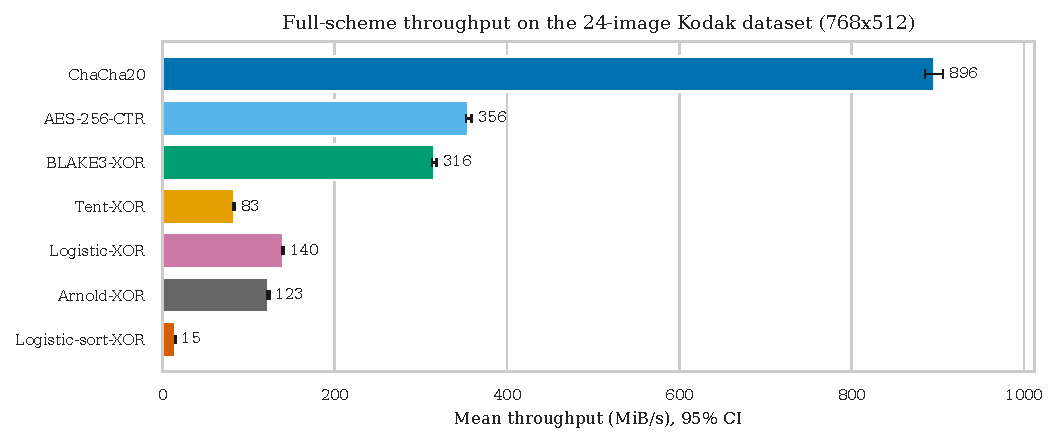
\includegraphics[width=\columnwidth]{full_scheme_throughput.pdf}
\caption{Selected full-scheme throughput on the 24-image Kodak dataset. Error
bars show 95\% confidence intervals. Standard cryptographic baselines remain
substantially faster than the evaluated chaotic full schemes.}
\label{fig:full-throughput}
\end{figure}

\subsection{Isolated Permutation Performance}
Permutation produces the largest stage-level improvement. At
512$\times$512, block permutation reaches 512.371 MiB/s and is 100.634 times
faster than chaotic sort. At 1024$\times$1024 it reaches 497.839 MiB/s and is
131.861 times faster.

\begin{table*}[t]
\caption{Block-Permutation Performance Relative to Chaotic Sort}
\label{tab:permutation}
\centering
\setlength{\tabcolsep}{3pt}
\begin{tabular}{lrrrr}
\toprule
\textbf{Size} & $\boldsymbol{n}$ & \textbf{MiB/s} & \textbf{CI} & \textbf{Speedup} \\
\midrule
512$\times$512 & 30 & 512.371 & 6.473 & 100.634$\times$ \\
512$\times$768 & 60 & 499.309 & 4.729 & 110.013$\times$ \\
768$\times$512 & 180 & 499.812 & 2.866 & 109.371$\times$ \\
1024$\times$1024 & 30 & 497.839 & 5.289 & 131.861$\times$ \\
\bottomrule
\end{tabular}
\end{table*}

This result answers RQ1 and RQ2: chaotic sort is implementation-hostile, and
replacing it with a regular linear-time transform changes the performance
regime. The benchmark block permutation is fixed and must be made key-derived
and cryptographically analyzed before use in a cipher.

\subsection{Isolated Diffusion Performance}
The fastest diffusion alternatives are multi-lane chaining and tree XOR.
Their mean speedups over the global chain are approximately twofold.

\begin{table*}[t]
\caption{Selected Aggregate Diffusion Performance}
\label{tab:diffusion}
\centering
\begin{tabular}{lrrrrr}
\toprule
\textbf{Stage} & \textbf{Image size} & $\boldsymbol{n}$ & \textbf{Mean MiB/s} & \textbf{95\% CI} & \textbf{Speedup} \\
\midrule
Multi-lane chain AVX2 & 512$\times$512 & 30 & 499.419 & 7.774 & 2.076$\times$ \\
Multi-lane chain AVX2 & 768$\times$512 & 180 & 499.120 & 3.046 & 2.095$\times$ \\
Multi-lane chain AVX2 & 1024$\times$1024 & 30 & 493.067 & 8.000 & 2.054$\times$ \\
Tree XOR AVX2 & 512$\times$512 & 30 & 470.202 & 7.667 & 1.955$\times$ \\
Tree XOR AVX2 & 768$\times$512 & 180 & 469.901 & 2.793 & 1.973$\times$ \\
Tree XOR AVX2 & 1024$\times$1024 & 30 & 464.386 & 8.035 & 1.935$\times$ \\
ARX block diffusion & 768$\times$512 & 180 & 426.568 & 2.540 & 1.791$\times$ \\
\bottomrule
\end{tabular}
\end{table*}

Removing a global byte-to-byte dependency creates a measurable SIMD
opportunity. It also explains why adding SIMD only to XOR inside a traditional
end-to-end pipeline may show little total improvement: the remaining generator
and permutation costs dominate.

\begin{figure}[t]
\centering
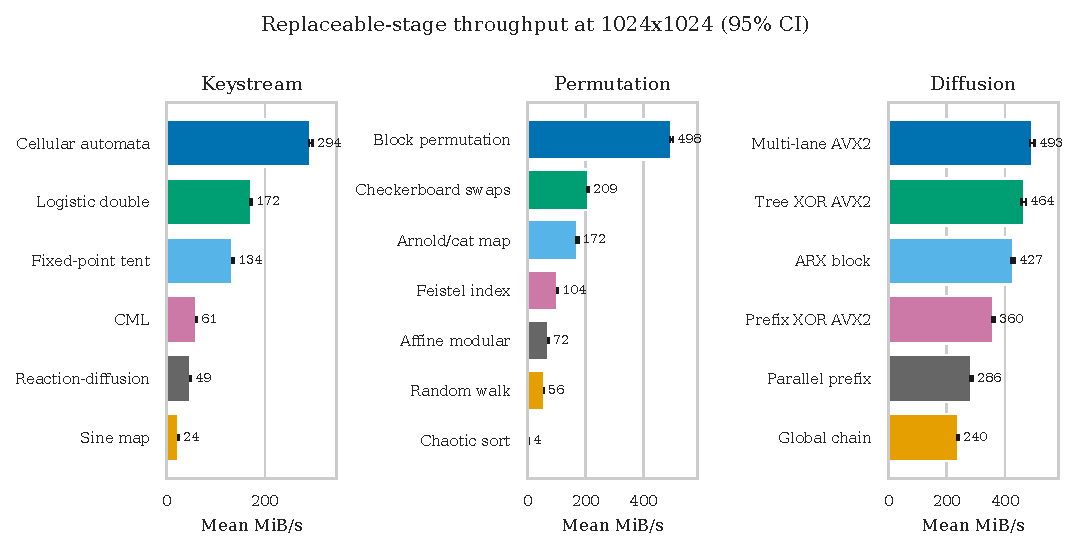
\includegraphics[width=\columnwidth]{stage_throughput_1024.pdf}
\caption{Representative replaceable-stage throughput at
1024$\times$1024. The largest gain is algorithmic: replacing chaotic sort with
a regular linear-time permutation. AVX2-native multi-lane and tree diffusion
also outperform the sequential global chain.}
\label{fig:stage-throughput}
\end{figure}

\begin{figure}[t]
\centering
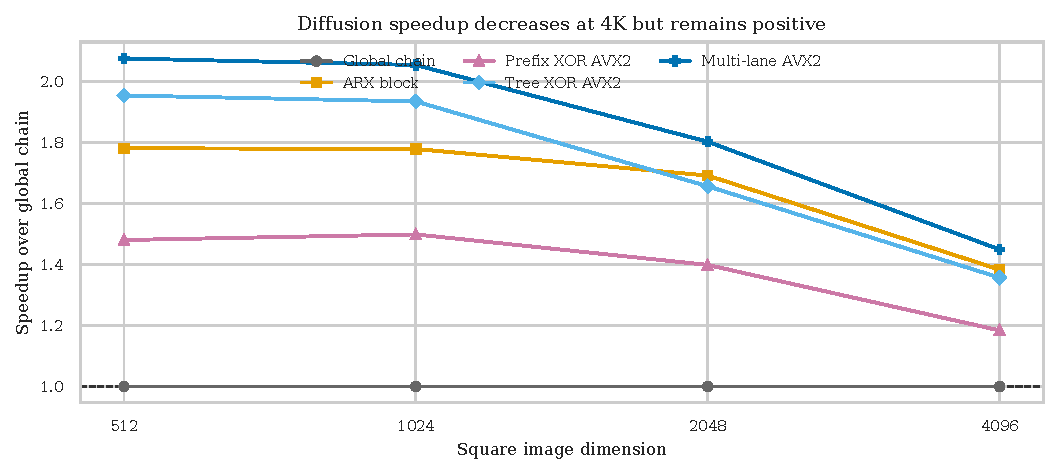
\includegraphics[width=\columnwidth]{diffusion_speedup.pdf}
\caption{Diffusion speedup relative to the global chain on square images.
AVX2 multi-lane and tree diffusion retain a positive advantage at all measured
sizes, although the advantage narrows at 4096$\times$4096.}
\label{fig:diffusion-speedup}
\end{figure}

\subsection{Candidate Pipeline Performance}
Checkerboard-CA-ARX is the fastest composed candidate. On Kodak images it
achieves 259.138 MiB/s, while Checkerboard-CA-MultilaneTree achieves
232.142 MiB/s. Both remain slower than AES-256-CTR and ChaCha20 on the same
image dimensions.

\begin{table*}[t]
\caption{Aggregate Candidate-Pipeline Throughput}
\label{tab:candidate-throughput}
\centering
\begin{tabular}{lrrrr}
\toprule
\textbf{Candidate} & \textbf{Image size} & $\boldsymbol{n}$ & \textbf{Mean MiB/s} & \textbf{95\% CI} \\
\midrule
Checkerboard-CA-ARX & 512$\times$512 & 30 & 267.596 & 3.771 \\
Checkerboard-CA-ARX & 768$\times$512 & 180 & 259.138 & 2.666 \\
Checkerboard-CA-ARX & 1024$\times$1024 & 30 & 234.149 & 4.490 \\
Checkerboard-CA-ARX & 2048$\times$2048 & 30 & 216.487 & 3.933 \\
Checkerboard-CA-ARX & 4096$\times$4096 & 30 & 199.993 & 4.384 \\
Checkerboard-CA-MultilaneTree & 768$\times$512 & 180 & 232.142 & 2.111 \\
Checkerboard-CA-MultilaneTree & 4096$\times$4096 & 30 & 159.392 & 3.931 \\
\bottomrule
\end{tabular}
\end{table*}

Table~\ref{tab:shares} shows that the fast checkerboard candidates distribute
work across all three stages, whereas Feistel indexing dominates
CA-Feistel-ARX and Hamiltonian generation dominates
Hamiltonian-Block-Stencil. These results support RQ3: isolated-stage choices
remain visible after composition.

\begin{figure}[t]
\centering
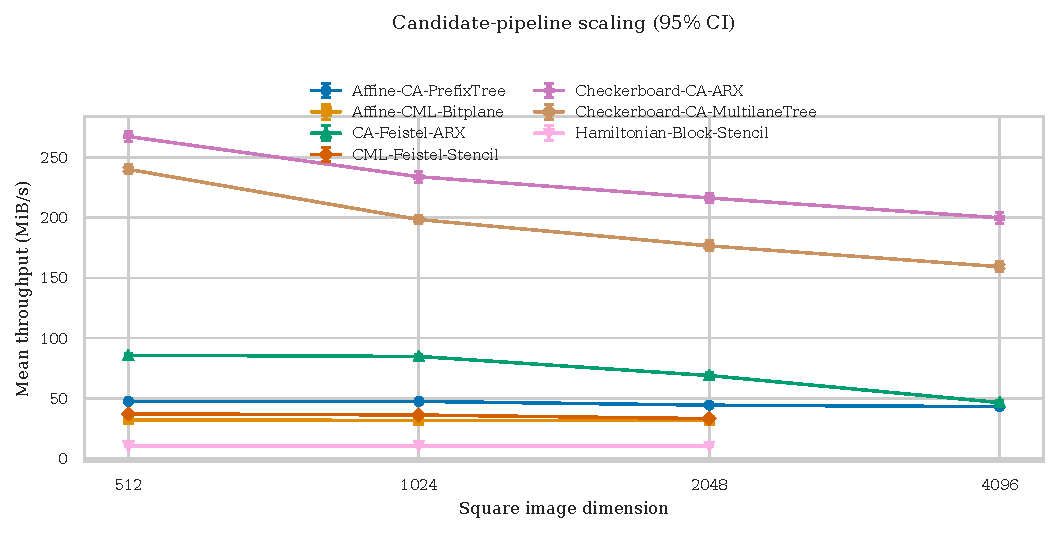
\includegraphics[width=\columnwidth]{candidate_scaling.pdf}
\caption{Candidate-pipeline throughput across square image sizes. The
checkerboard candidates remain fastest, but all candidates lose throughput as
working sets grow. Error bars show 95\% confidence intervals.}
\label{fig:candidate-scaling}
\end{figure}

\begin{table*}[t]
\caption{Mean Candidate Stage Shares}
\label{tab:shares}
\centering
\setlength{\tabcolsep}{2.5pt}
\begin{tabular}{lrrr}
\toprule
\textbf{Candidate} & \textbf{Key} & \textbf{Perm.} & \textbf{Diff.} \\
\midrule
Checkerboard-CA-ARX & 47.69\% & 27.86\% & 24.44\% \\
Checkerboard-CA-MultilaneTree & 38.44\% & 22.60\% & 38.95\% \\
CA-Feistel-ARX & 11.69\% & 82.32\% & 5.99\% \\
Hamiltonian-Block-Stencil & 83.78\% & 11.97\% & 4.24\% \\
\bottomrule
\end{tabular}
\end{table*}

\begin{figure}[t]
\centering
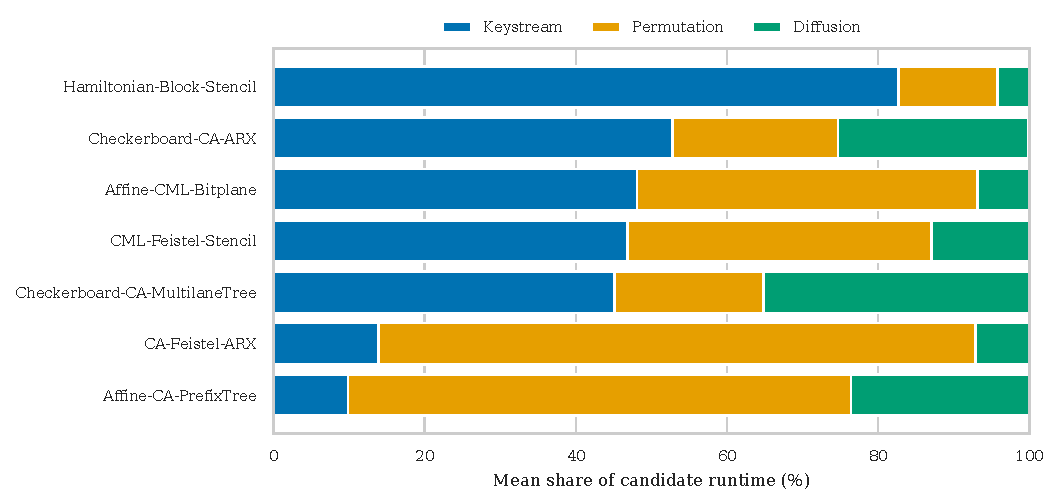
\includegraphics[width=\columnwidth]{candidate_stage_shares.pdf}
\caption{Mean runtime composition of the candidate pipelines. The plot exposes
the dominant bottleneck in each composition and shows why isolated stage
measurements remain necessary.}
\label{fig:candidate-shares}
\end{figure}

\subsection{Video-Frame Real-Time Feasibility}
The real-time extension reruns the benchmark on a public video-frame
workload at 1280$\times$720 and 1920$\times$1080. Each row in
Table~\ref{tab:realtime-video} summarizes 36 measurements for the corresponding
scheme, resolution, and architecture. The x86-64 run used the local Xeon host;
the ARM64 run used an AWS aarch64 host. The table is intentionally a
feasibility check rather than a deployment guarantee because complete
real-time systems must also budget capture, transport, display, storage,
authentication, and downstream processing.

\begin{table*}[t]
\caption{Video-Frame Real-Time Feasibility on x86-64 and ARM64}
\label{tab:realtime-video}
\centering
\tiny
\setlength{\tabcolsep}{1.5pt}
\begin{tabular}{@{}llrrrrcc@{}}
\toprule
\textbf{Arch.} & \textbf{Scheme} & \textbf{Res.} &
\textbf{Mean} & \textbf{p95} & $\boldsymbol{\mathrm{FPS}_{eq}}$ &
\textbf{30} & \textbf{60} \\
\midrule
x86-64 & Ckbd-CA-ARX & 1280$\times$720 & 12.77 & 14.06 & 78.30 & yes & yes \\
x86-64 & Ckbd-CA-ARX & 1920$\times$1080 & 28.99 & 31.06 & 34.49 & yes & no \\
x86-64 & AES-GCM & 1280$\times$720 & 3.02 & 3.44 & 330.59 & yes & yes \\
x86-64 & AES-GCM & 1920$\times$1080 & 7.82 & 8.43 & 127.82 & yes & yes \\
x86-64 & ChaCha20 & 1280$\times$720 & 3.28 & 3.56 & 304.72 & yes & yes \\
x86-64 & ChaCha20 & 1920$\times$1080 & 8.44 & 9.39 & 118.55 & yes & yes \\
ARM64 & Ckbd-CA-ARX & 1280$\times$720 & 5.44 & 5.87 & 183.85 & yes & yes \\
ARM64 & Ckbd-CA-ARX & 1920$\times$1080 & 12.01 & 12.84 & 83.24 & yes & yes \\
ARM64 & AES-GCM & 1280$\times$720 & 1.88 & 2.06 & 531.20 & yes & yes \\
ARM64 & AES-GCM & 1920$\times$1080 & 4.06 & 4.12 & 246.59 & yes & yes \\
ARM64 & ChaCha20 & 1280$\times$720 & 3.19 & 3.39 & 313.92 & yes & yes \\
ARM64 & ChaCha20 & 1920$\times$1080 & 7.01 & 7.20 & 142.71 & yes & yes \\
\bottomrule
\end{tabular}
\footnotetext{Ckbd-CA-ARX denotes Checkerboard-CA-ARX. Mean and p95 are in milliseconds per frame.}
\end{table*}

These results answer RQ4 for the measured hosts. The fastest chaotic candidate
meets 30 FPS at both video resolutions on both architectures. It meets 60 FPS
at 720p on x86-64 and at both resolutions on the measured ARM64 host, but it
misses the 60 FPS threshold at 1080p on the x86-64 host. The standardized
cryptographic baselines remain faster and meet both frame-rate thresholds in
all measured video-frame cases.

\subsection{Cross-Architecture Reproducibility}
To check whether the conclusions depend on one CPU family, the publication
harness was rerun on the local Intel Xeon E5-2620 v4 host with AVX2 and on an
AWS aarch64 host. The matched run used synthetic sizes
256, 512, and 1024, three repetitions, one warm-up, four timed iterations, and
the Kodak pair \texttt{kodim01.png} and \texttt{kodim02.png}. The paired
geometric-mean analysis over five images preserved the same qualitative
ordering on both systems: \texttt{scan\_exact} consistently beat the scalar
chain for the map and symbolic families, while \texttt{sort\_logistic}
remained near parity.

\begin{table*}[t]
\caption{Representative Cross-Architecture Paired Speedups}
\label{tab:cross-arch}
\centering
\setlength{\tabcolsep}{3pt}
\begin{tabular}{lcc}
\toprule
\textbf{Case} & \textbf{x86} & \textbf{ARM} \\
\midrule
Map + scan exact & 1.166$\times$ / 1.074$\times$ & 1.305$\times$ / 1.103$\times$ \\
Symbolic + scan exact & 1.153$\times$ / 1.053$\times$ & 1.308$\times$ / 1.115$\times$ \\
Bitplane + scan exact & 1.101$\times$ / 0.933$\times$ & 1.249$\times$ / 1.068$\times$ \\
Sort logistic + scan exact & 1.032$\times$ / 1.012$\times$ & 1.042$\times$ / 1.016$\times$ \\
\bottomrule
\end{tabular}
\end{table*}

These paired runs support the claim that the main throughput ranking is not an
artifact of the Xeon server alone. The exact-scan variant is the most robust
replacement across both architectures, even though the absolute gains differ
slightly by host and stage family.

\subsection{Recent Literature Positioning}
The recent chaos-based image-encryption literature still emphasizes
confusion-diffusion compositions, hybrid key schedules, geometric block
permutation, and statistical security diagnostics. Representative recent
examples include multithreaded parallel confusion and diffusion for video
frames \cite{jiang2023}, a medical-imagery permutation-diffusion design
\cite{sanaboina2024}, geometric block permutation with dynamic substitution
\cite{ali2025}, and data-identified discrete chaotic maps \cite{li2026}.

\begin{table*}[t]
\caption{Representative Recent Works and the Remaining Measurement Gap}
\label{tab:recent-work}
\centering
\setlength{\tabcolsep}{4pt}
\begin{tabular}{p{0.08\textwidth}p{0.36\textwidth}p{0.22\textwidth}p{0.24\textwidth}}
\toprule
\textbf{Year} & \textbf{Representative work} & \textbf{Family / emphasis} & \textbf{Gap relative to this paper} \\
\midrule
2023 & \cite{jiang2023} & Multithreaded parallel confusion-diffusion for video frames & Reports speed and statistical tests, but not stage-level attribution across architectures. \\
2024 & \cite{sanaboina2024} & Chaos-based permutation-diffusion for diagnostic imagery & Focuses on image statistics and functional encryption, not SIMD stage decomposition. \\
2025 & \cite{ali2025} & Geometric block permutation with dynamic substitution & Emphasizes statistical security, not finite-precision or cross-CPU benchmarking. \\
2026 & \cite{li2026} & Data-identified discrete chaotic maps & Explores a newer map family, but still centers on cipher statistics rather than stage timing. \\
\bottomrule
\end{tabular}
\end{table*}

These selected works illustrate the measurement gap addressed here: recent
papers continue to emphasize cipher structure and image-domain statistics,
whereas the present study focuses on measured implementation cost,
stage-level attribution, and cross-architecture reproducibility.

\subsection{Full-Scheme Security Diagnostics}
All complete schemes decrypt correctly. Several also produce near-eight-bit
entropy, low adjacent-pixel correlation, and strong key sensitivity. These
positive metrics are insufficient to establish security.

\begin{table*}[t]
\caption{Mean Security Diagnostics Across 300 Observations per Scheme}
\label{tab:security}
\centering
\setlength{\tabcolsep}{4pt}
\begin{tabular}{lrrrrrr}
\toprule
\textbf{Scheme} & \textbf{Entropy} & $\boldsymbol{\chi^2}$ & \textbf{Abs. corr.} & \textbf{Flip NPCR} & \textbf{Key sens.} & \textbf{KPA} \\
\midrule
ChaCha20 & 7.999845 & 258.874 & 0.001216 & 0.000084\% & 99.619\% & 1.000 \\
AES-256-CTR & 7.999843 & 259.125 & 0.001148 & 0.000084\% & 99.611\% & 1.000 \\
BLAKE3-XOR & 7.999850 & 247.607 & 0.001419 & 0.000084\% & 99.607\% & 1.000 \\
Tent-XOR & 7.999828 & 282.731 & 0.001721 & 0.000084\% & 99.623\% & 1.000 \\
Logistic-XOR & 7.984321 & 26641.399 & 0.020440 & 0.000084\% & 99.387\% & 1.000 \\
Coupled-lattice-XOR & 7.971770 & 45857.479 & 0.137337 & 0.000084\% & 99.410\% & 1.000 \\
\bottomrule
\end{tabular}
\end{table*}

Here, \emph{Flip NPCR} denotes a one-bit plaintext-flip diagnostic measured
under a fixed key/nonce. The KPA recovery score of 1.0 for AES-CTR, ChaCha20,
BLAKE3-XOR, and the
stream-XOR chaotic variants is expected because the experiment deliberately
reuses the same key/nonce. It demonstrates misuse sensitivity, not a break of
the underlying standardized primitive. The negligible plaintext NPCR is also
expected for CTR- or stream-XOR encryption: changing one plaintext bit changes
only the corresponding ciphertext bit when the keystream is unchanged.

This result answers RQ5. Entropy, correlation, and key sensitivity can look
excellent while a construction still lacks plaintext avalanche and fails
under reused keystream. NPCR is not an appropriate requirement for all secure
encryption modes; standard stream ciphers intentionally do not provide
plaintext avalanche. The candidate pipelines were not subjected to the same
security harness and contain fixed prototype permutations. No
cryptographic-security conclusion is made for them.

\subsection{Negative-Control Summary}
The control probes below are the ones reviewers usually ask for when a chaos
paper leans too hard on image statistics. They are useful precisely because
they do not prove security: they expose misuse sensitivity, limited avalanche
under keystream reuse, and the missing finite-precision analysis.

\begin{table*}[t]
\caption{Negative-Control Outcomes}
\label{tab:negative-controls}
\centering
\setlength{\tabcolsep}{4pt}
\begin{tabular}{p{0.22\textwidth}p{0.30\textwidth}p{0.38\textwidth}}
\toprule
\textbf{Control} & \textbf{Measured outcome} & \textbf{Interpretation} \\
\midrule
Reused key/nonce & KPA recovery score is 1.000 for ChaCha20, AES-CTR, BLAKE3-XOR, Tent-XOR, Logistic-XOR, and Coupled-lattice-XOR. & This is a misuse probe. It shows deterministic recovery under repeated keystream, not a break of the underlying primitive. \\
One-bit plaintext flip & NPCR is 0.000084\% for the same full-scheme controls. & Stream and CTR-style constructions do not provide plaintext avalanche under keystream reuse; this is the expected control result. \\
One-bit key flip & Key sensitivity stays in the 99.387--99.623\% range across the measured full schemes. & Sensitivity is high but still only a diagnostic, not a security proof. \\
Finite precision orbit collapse & Exact double logistic orbits showed no repeat within $10^6$ steps across 16 seeds. The 16-bit quantized logistic stress test repeated in all 16 seeds after 35--549 steps (median 161; cycle length 5--245, median 60). The fixed-point tent probe also showed no repeat within $10^6$ steps. & Finite precision clearly changes effective orbit length; the exact implementation still needs a longer-horizon orbit-length or state-space study before any stronger claim. \\
\bottomrule
\end{tabular}
\end{table*}

The finite-precision row is deliberate: it now records a reduced-precision
stress test instead of leaving the analysis blank. The exact double orbit
still only gives a lower bound on repeat length, which is the correct level of
claim for this harness.

\begin{figure}[t]
\centering
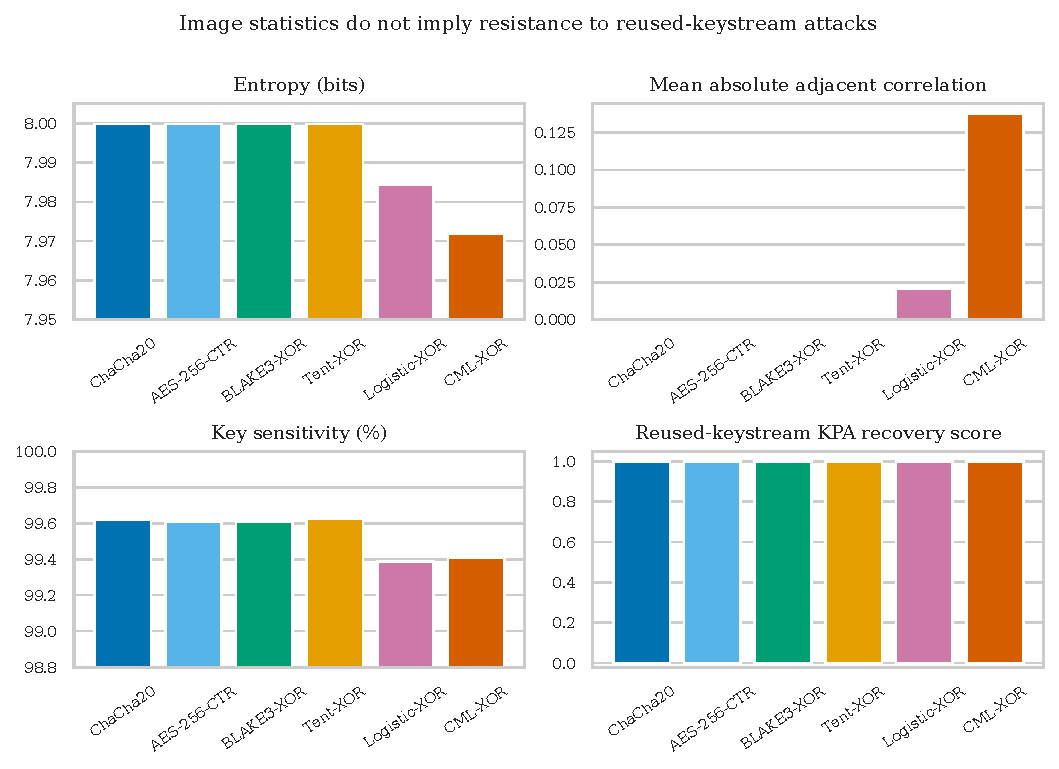
\includegraphics[width=\columnwidth]{security_diagnostics.pdf}
\caption{Selected security diagnostics averaged over the full-scheme
experiments. Near-ideal entropy, correlation, and key sensitivity coexist with
complete recovery in the deliberately reused-keystream known-plaintext probe.}
\label{fig:security-diagnostics}
\end{figure}

\section{Discussion}
\label{sec:discussion}

\subsection{What SIMD Changes}
The experiments show that SIMD is not a property of a pipeline label. It is a
property of the dependency graph and memory-access pattern of each stage.
Regular, independent byte or word operations benefit from AVX2. Global
recurrences, transcendental scalar maps, cycle walking, and sort-based
permutation restrict the gain.

The largest improvement does not come from a vector instruction alone. It
comes from replacing chaotic sort with a linear regular mapping. Similarly,
the diffusion improvement comes from changing one global chain into multiple
lanes or a tree. Algorithmic restructuring precedes vectorization.

\subsection{Performance Versus Security}
The fastest stage is not necessarily the strongest stage. Fixed block and
checkerboard permutations are useful controls for measuring the cost of
regular memory movement, but they provide no secret permutation by themselves.
The CA generator is fast, but its rule-30-like output has not been established
as a cryptographically secure pseudorandom stream. Tree XOR and linear
multi-lane diffusion are also structurally analyzable.

A deployment-oriented design requires a standard cryptographic primitive to
derive independent subkeys and masks, make every permutation key-derived,
include unique nonces, and provide authentication. A practical research
direction is to retain image-domain transforms only as a format-aware
preprocessing or selective-encryption layer, then protect the result with an
authenticated standard cipher.

\subsection{Implications for Future Studies}
Future evaluations need to report isolated stage execution time; include AES
and ChaCha through optimized libraries; compare algorithmic complexity before
attributing speedup to SIMD; test real images, controlled synthetic inputs,
and public video-frame workloads; report repeated measurements with confidence
intervals and p95 frame latency; separate image statistics from cryptographic
claims; and include negative controls for nonce reuse, known plaintext, and
chosen plaintext.

\section{Threats to Validity and Limitations}
\label{sec:limitations}
Measurements were collected on one older x86-64 server CPU and one ARM64 cloud
host, and may differ on newer AVX2/AVX-512 processors, ARM NEON/SVE systems,
GPUs, or embedded devices. The reported x86/ARM video-frame run checks whether
the main ranking survives across two CPU families, but it is not a full
hardware survey. The ARM64 metadata does not retain cloud instance type, memory
size, or frequency-governor state. CPU frequency, virtualization noise, memory
allocation, and cache state were not controlled through hardware performance
counters or processor pinning. The benchmark reports wall-clock stage time and
throughput, but not cycles per byte, energy, cache misses, branch misses, or
instruction counts.

The prefix-XOR helper is only partially vectorized because its intra-vector
scan is scalar. BLAKE3 is compiled without architecture-specific SIMD
dispatch. Fixed block and checkerboard permutations are performance templates,
not secure key-derived permutations. Candidate pipelines do not yet implement
inverse transforms or undergo the full cryptanalysis suite. Image-domain
diagnostics are reported only for full schemes and do not constitute proofs of
security. AES-CTR and ChaCha20 are confidentiality-only baselines; deployment
requires authenticated encryption. Finite-precision state-collapse is covered
only as a reduced-precision stress test, and a longer-horizon exact
orbit-length study is still needed before any stronger claim about the chaotic
maps themselves.

These limitations constrain the claim to stage-level performance analysis and
prototype composition. They do not invalidate the finding that sort
permutation and global dependencies are major implementation bottlenecks.

\section{Reproducibility}
\label{sec:reproducibility}
The public research artifact is maintained on GitHub as
\texttt{chaotic-encryption-survey}. The repository includes the benchmark
implementation, dataset generators, Kodak
downloader, experiment harness, raw outputs, aggregate CSV files,
figure-generation scripts, and manuscript source. After cloning the public
artifact repository, a clean checkout can be built and the final experiment
reproduced with:
\begin{verbatim}
cd chaotic-encryption-survey
cmake -S . -B build \
  -DCMAKE_BUILD_TYPE=Release
cmake --build build -j
REPS=10 REAL_REPS=10 \
SIZES="512 1024 2048 4096" \
./scripts/run_paper_ready_experiments.sh
\end{verbatim}
Primary result files include \path{results/final/bench.csv},
\path{stage_bench.csv}, \path{candidate_schemes.csv}, \path{analysis.csv},
\path{dataset_manifest.csv}, and their aggregate statistics. The repository
README documents dependencies, quick-start commands, plot generation, and
manuscript compilation. The complete source revision used by each experiment
is retained in the generated metadata.

The JRTIP real-time extension is reproduced with \texttt{RUN\_VIDEO=1} and
separate output directories for the x86-64 and ARM64 hosts. The committed
result-data directories are \path{results/jrtip_realtime} and
\path{results/jrtip_realtime_arm}; they contain CSV and Markdown measurements
only, not generated ciphertext images or downloaded datasets.

\section{Conclusion}
\label{sec:conclusion}
This work decomposed chaotic image-encryption pipelines into replaceable
keystream, permutation, and diffusion stages and evaluated traditional and
SIMD-oriented alternatives under a real-time-oriented measurement model.
Implementation-hostile components, especially chaotic sort and global feedback
dependencies, determine encryption latency and throughput more strongly than
the mere use of SIMD instructions.

Linear block permutation improves throughput by more than two orders of
magnitude relative to chaotic sort. AVX2 multi-lane and tree diffusion
approximately double throughput relative to a global chain. These improvements
remain visible in composed candidate pipelines and at resolutions up to
4096$\times$4096. Nevertheless, optimized ChaCha20 and AES-256-CTR remain
faster and have substantially stronger security foundations.

For a real-time image-processing venue, the central implementation lesson is
that stage-level timing must be converted into frame-level feasibility:
milliseconds per frame, FPS-equivalent throughput, p95 video-frame latency,
and pass/fail status against 30/60 FPS budgets. The results include a
public 720p/1080p video-frame workload on both x86-64 and ARM64. They show
that Checkerboard-CA-ARX meets 30 FPS at both resolutions on both measured
hosts, while optimized AES-GCM and ChaCha20 remain faster and meet both
30 FPS and 60 FPS thresholds in the measured video-frame cases.

The security experiments reinforce an equally important conclusion:
image-domain statistics must not be presented as cryptographic proof. The
XOR-based full schemes show favorable entropy and key sensitivity but fail
differential-avalanche and reused-keystream recovery controls. The
benchmark-informed candidates are therefore performance prototypes, not secure
ciphers.


\section*{Declarations}

\subsection*{Funding}
No external funding was received for this study.

\subsection*{Conflict of interest}
The author declares no competing interests.

\subsection*{Ethics approval and consent to participate}
Not applicable. The study uses public image/video benchmark data and synthetic images; it does not involve human participants, animals, or private personal data.

\subsection*{Consent for publication}
Not applicable.

\subsection*{Data availability}
The benchmark source code, experiment scripts, raw measurements, aggregate tables, manuscript source, and reproduction instructions are available in the public GitHub repository \texttt{chaotic-encryption-survey}. The committed JRTIP result directories contain CSV and Markdown measurements only; generated ciphertext images and downloaded datasets are excluded from version control.

\subsection*{Code availability}
The benchmark implementation and scripts are available in the same public repository.

\subsection*{Author contribution}
Ravikanth Reddy Gudipati conceived the study, implemented the benchmark, conducted the experiments, analyzed the results, and prepared the manuscript.

\subsection*{Use of generative AI and AI-assisted technologies}
Generative-AI and large-language-model tools were used for editorial and engineering assistance during preparation of this manuscript and research artifact. The assistance included prose reorganization, claim-boundary review, LaTeX macro-package conversion support, and suggestions for reproducibility documentation and small automation scripts. The author reviewed all generated text and code suggestions, ran or inspected the reported experiments, verified numerical claims against committed result files, and takes full responsibility for the final manuscript and artifact.

\begin{thebibliography}{00}
\bibitem{shannon1949} C. E. Shannon, ``Communication theory of secrecy
systems,'' \emph{Bell System Technical Journal}, vol. 28, no. 4,
pp. 656--715, 1949, doi: 10.1002/j.1538-7305.1949.tb00928.x.

\bibitem{fridrich1998} J. Fridrich, ``Symmetric ciphers based on
two-dimensional chaotic maps,'' \emph{International Journal of Bifurcation
and Chaos}, vol. 8, no. 6, pp. 1259--1284, 1998,
doi: 10.1142/S021812749800098X.

\bibitem{fu2014} C. Fu, J.-B. Huang, N.-N. Wang, Q.-B. Hou, and W.-M. Lei,
``A symmetric chaos-based image cipher with an improved bit-level permutation
strategy,'' \emph{Entropy}, vol. 16, no. 2, pp. 770--788, 2014,
doi: 10.3390/e16020770.

\bibitem{huang2018} L. Huang, S. Cai, M. Xiao, and X. Xiong, ``A simple
chaotic map-based image encryption system using both plaintext related
permutation and diffusion,'' \emph{Entropy}, vol. 20, no. 7, Art. no. 535,
2018, doi: 10.3390/e20070535.

\bibitem{chai2015} X. Chai \emph{et al.}, ``A new color image encryption
scheme using CML and a fractional-order chaotic system,'' \emph{PLoS ONE},
vol. 10, no. 3, Art. no. e0119660, 2015,
doi: 10.1371/journal.pone.0119660.

\bibitem{zhang2023} W. Zhang, Y. Wang, and K. A. Ross, ``Parallel prefix sum
with SIMD,'' arXiv:2312.14874, 2023, doi: 10.48550/arXiv.2312.14874.

\bibitem{wu2011} Y. Wu, J. P. Noonan, and S. Agaian, ``NPCR and UACI
randomness tests for image encryption,'' \emph{Journal of Selected Areas in
Telecommunications}, pp. 31--38, 2011.

\bibitem{li2018} C. Li, D. Lin, B. Feng, J. L\"u, and F. Hao,
``Cryptanalysis of a chaotic image encryption algorithm based on information
entropy,'' \emph{IEEE Access}, vol. 6, pp. 75834--75842, 2018,
doi: 10.1109/ACCESS.2018.2883690.

\bibitem{jiang2023} D. Jiang, Z. Yuan, W. Li, and L. Lu, ``Real-time chaotic
video encryption based on multithreaded parallel confusion and diffusion,''
\emph{arXiv preprint arXiv:2302.07411}, 2023. [Online]. Available:
\url{https://arxiv.org/abs/2302.07411}

\bibitem{sanaboina2024} C. S. Sanaboina and T. Yadla, ``An effective approach
to scramble multiple diagnostic imageries using chaos-based cryptography,''
\emph{arXiv preprint arXiv:2406.07560}, 2024. [Online]. Available:
\url{https://arxiv.org/abs/2406.07560}

\bibitem{ali2025} M. Ali \emph{et al.}, ``A chaotic image encryption scheme
using novel geometric block permutation and dynamic substitution,''
\emph{arXiv preprint arXiv:2503.09939}, 2025. [Online]. Available:
\url{https://arxiv.org/abs/2503.09939}

\bibitem{li2026} W. Li \emph{et al.}, ``Image encryption via data-identified
discrete chaotic maps,'' \emph{arXiv preprint arXiv:2605.21118}, 2026.
[Online]. Available: \url{https://arxiv.org/abs/2605.21118}

\bibitem{liu2015} Y. Liu, L. Y. Zhang, J. Wang, Y. Zhang, and K.-W. Wong,
``Chosen-plaintext attack of an image encryption scheme based on modified
permutation-diffusion structure,'' arXiv:1503.06638, 2015,
doi: 10.48550/arXiv.1503.06638.

\bibitem{nist2023} National Institute of Standards and Technology,
``Advanced Encryption Standard (AES),'' FIPS PUB 197, updated 2023,
doi: 10.6028/NIST.FIPS.197-upd1.

\bibitem{rfc8439} Y. Nir and A. Langley, ``ChaCha20 and Poly1305 for IETF
protocols,'' RFC 8439, 2018. [Online]. Available:
\url{https://www.rfc-editor.org/rfc/rfc8439}

\bibitem{blake3} J. O'Connor, J.-P. Aumasson, S. Neves, and
Z. Wilcox-O'Hearn, ``BLAKE3: One function, fast everywhere,'' 2020.
[Online]. Available:
\url{https://github.com/BLAKE3-team/BLAKE3-specs/blob/master/blake3.pdf}

\bibitem{kodak} R. Franzen, ``Kodak lossless true color image suite.''
[Online]. Available: \url{https://r0k.us/graphics/kodak/}
\end{thebibliography}

\end{document}
